\documentclass[border=8pt]{standalone}
\usepackage{pgfplots}
\usepgfplotslibrary{fillbetween, groupplots}
\usetikzlibrary{positioning, calc}
\pgfplotsset{compat=1.18}
\usepackage{amsmath}
\usepackage{graphicx}
\usepackage{xcolor}

\definecolor{algcol0}{HTML}{3B7BC8}
\definecolor{algcol1}{HTML}{7B6EBF}
\definecolor{algcol2}{HTML}{389C56}
\definecolor{algcol3}{HTML}{E63946}

\pgfplotsset{
  il plot/.style={
    width=5.8cm,
    height=5.8cm,
    grid=both,
    grid style={line width=0.35pt, draw=gray!35},
    xtick={1,2,3,5,7,10,30,50,100},
    xticklabel style={font=\normalsize},
    yticklabel style={font=\normalsize},
    ylabel style={font=\normalsize\bfseries, align=center},
    title style={font=\footnotesize},
  }
}

\begin{document}
  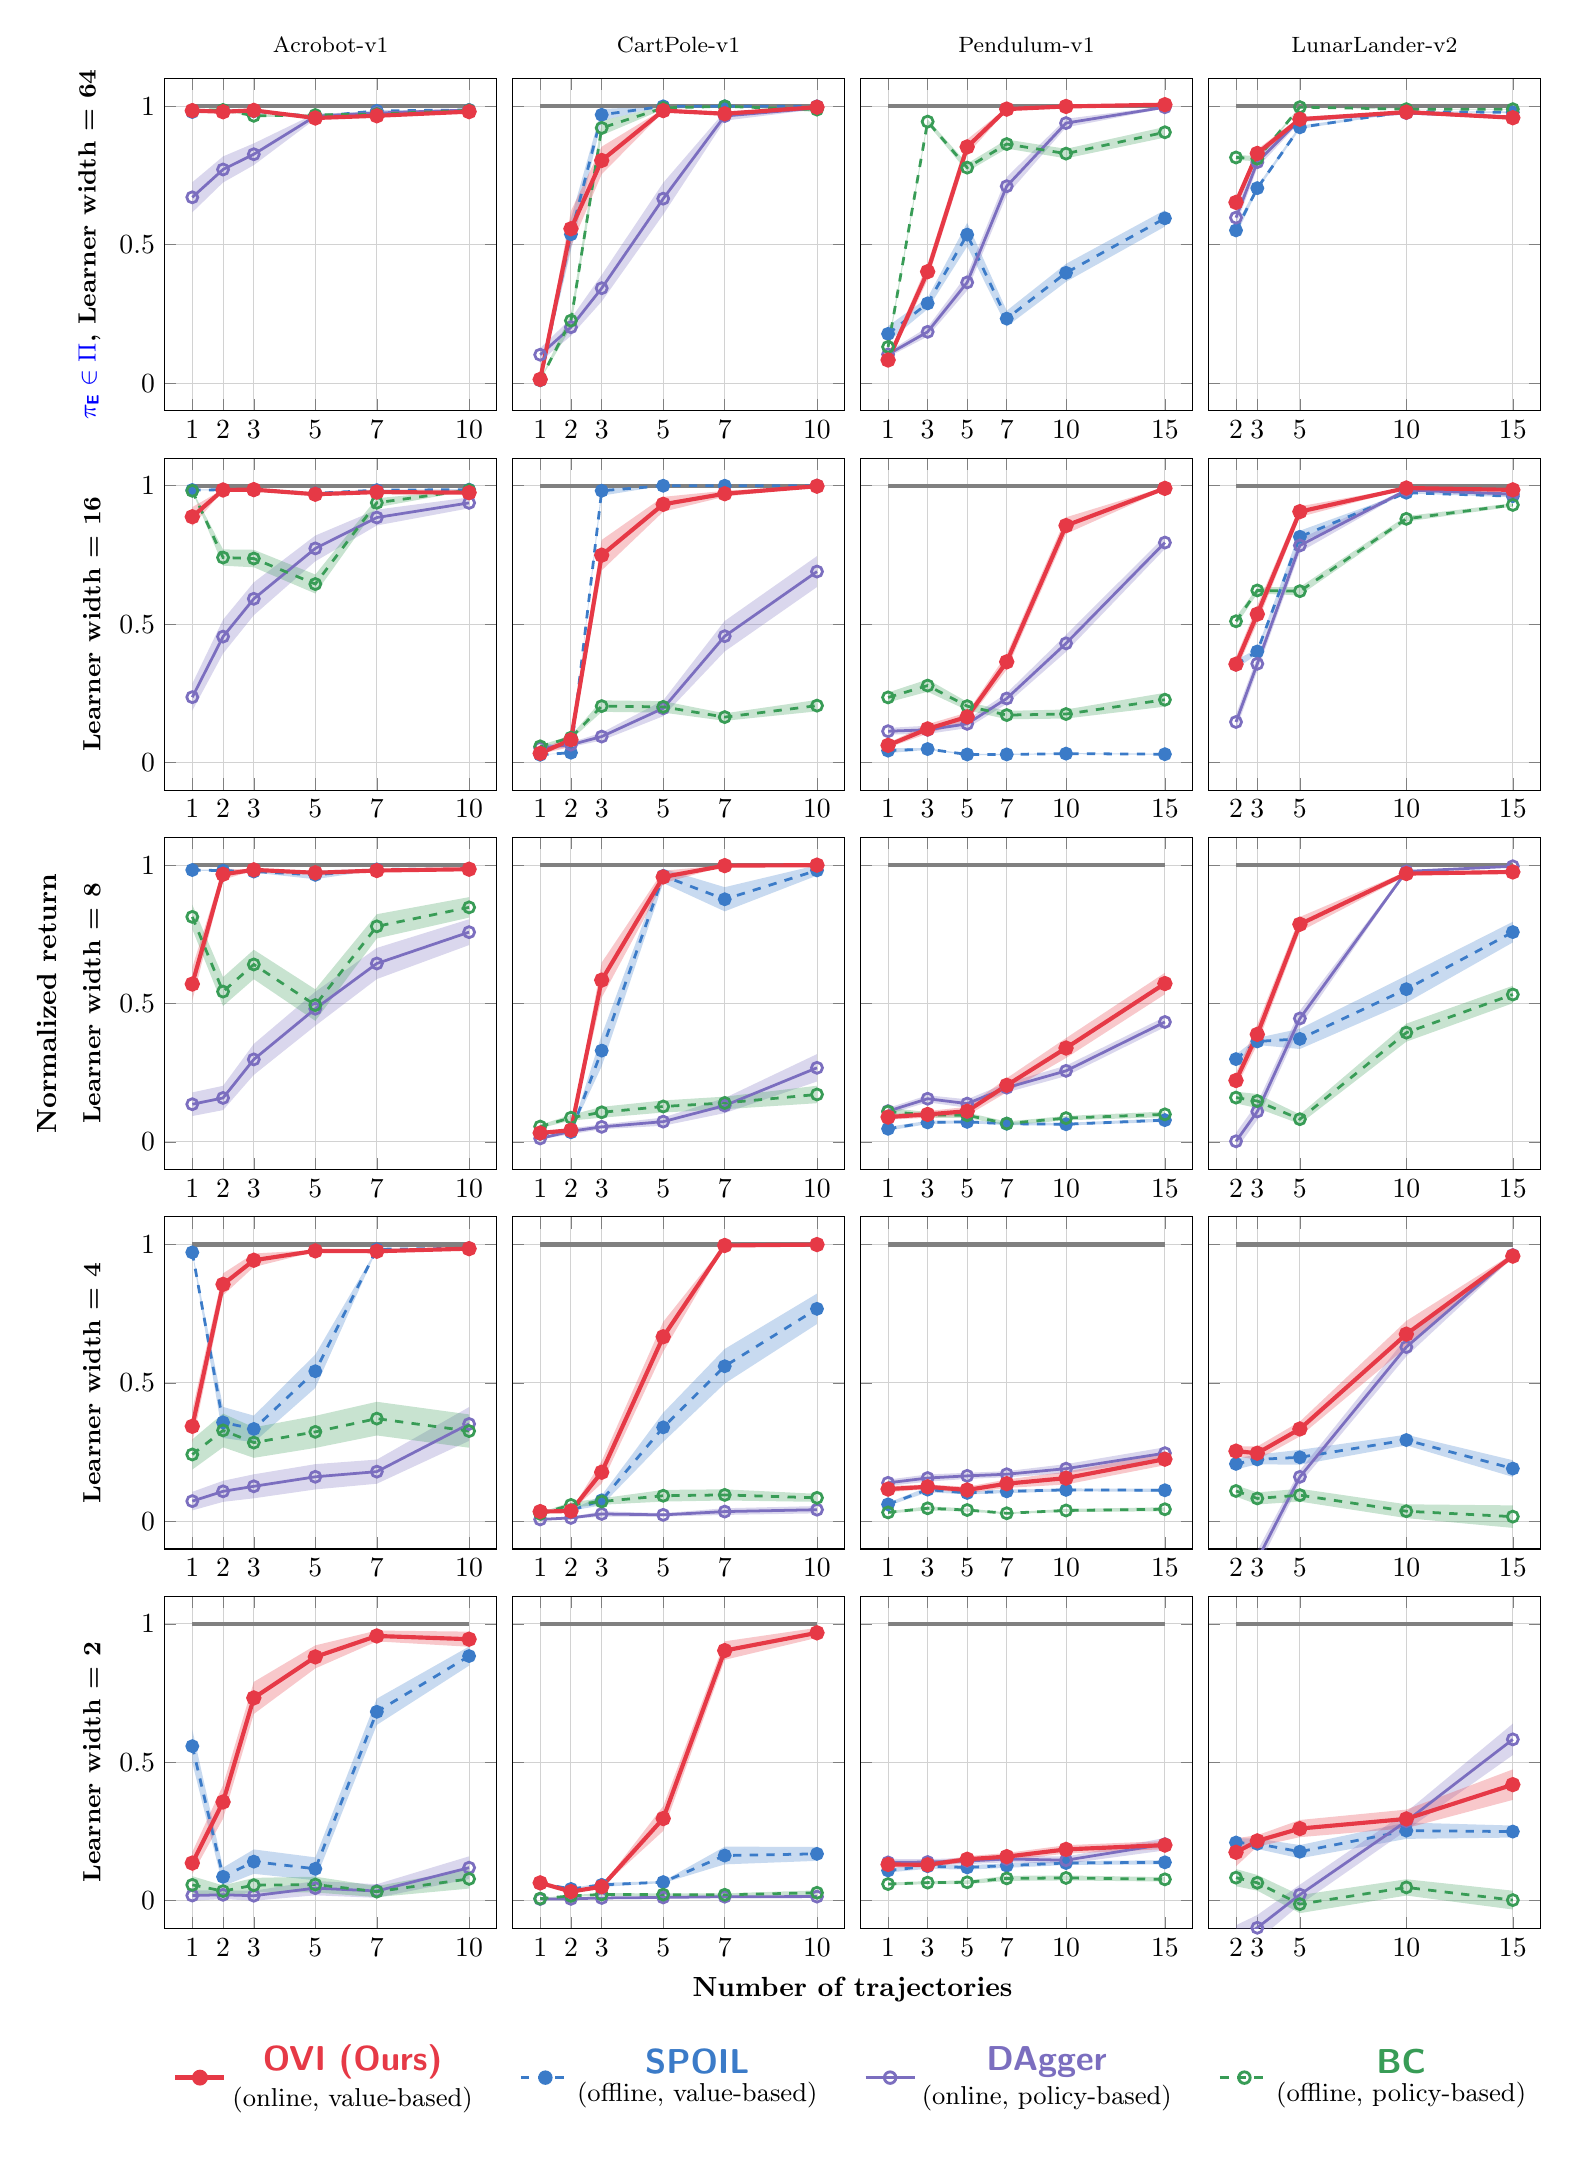
\begin{tikzpicture}
  \begin{groupplot}[
    il plot,
    group style={
      group size=4 by 5,
      horizontal sep=0.2cm,
      vertical sep=0.6cm,
      xlabels at=edge bottom,
      ylabels at=edge left,
    },
  ]
  \nextgroupplot[
    ymin=-0.1,
    ymax=1.1,
    title={Acrobot-v1},
    ylabel={{\small\textcolor{blue}{$\pi_{\textsf{E}} \in \Pi$}, Learner width = 64}},
    legend to name=sharedlegend,
    legend columns=4,
    legend style={draw=none,font=\small,/tikz/every even column/.append style={column sep=0.5cm}}
  ]
  \addlegendimage{algcol3, solid, mark=*, mark size=2.0pt, line width=1.5pt}
  \addlegendentry{\shortstack[c]{{\large\textcolor{algcol3}{\textbf{\textsf{OVI (Ours)}}}}\\(online, value-based)}}
  \addplot[gray, solid, line width=1.5pt, forget plot] coordinates { (1,1.00000) (10,1.00000) };
  % \shortstack[c]{{\large\textcolor{algcol0}{\textbf{\textsf{SPOIL}}}}\\(offline, value-based)}
  \addplot[name path=pu0, draw=none, forget plot] coordinates { (1,0.98164) (2,0.98553) (3,0.98417) (5,0.96732) (7,0.98575) (10,0.98851) };
  \addplot[name path=pl0, draw=none, forget plot] coordinates { (1,0.97723) (2,0.98047) (3,0.98018) (5,0.95854) (7,0.98155) (10,0.98539) };
  \addplot[fill=algcol0, fill opacity=0.28, draw=none, forget plot] fill between[of=pu0 and pl0];
  \addplot[algcol0, dashed, mark=*, mark size=2.0pt, line width=1.0pt, opacity=1.0, mark options={solid}] coordinates { (1,0.97943) (2,0.98300) (3,0.98218) (5,0.96293) (7,0.98365) (10,0.98695) };
  \addlegendentry{\shortstack[c]{{\large\textcolor{algcol0}{\textbf{\textsf{SPOIL}}}}\\(offline, value-based)}}
  % \shortstack[c]{{\large\textcolor{algcol1}{\textbf{\textsf{DAgger}}}}\\(online, policy-based)}
  \addplot[name path=pu1, draw=none, forget plot] coordinates { (1,0.72564) (2,0.81900) (3,0.86614) (5,0.97387) (7,0.97946) (10,0.98917) };
  \addplot[name path=pl1, draw=none, forget plot] coordinates { (1,0.61696) (2,0.72463) (3,0.78764) (5,0.95434) (7,0.97238) (10,0.98425) };
  \addplot[fill=algcol1, fill opacity=0.28, draw=none, forget plot] fill between[of=pu1 and pl1];
  \addplot[algcol1, solid, mark=o, mark size=2.0pt, line width=1.0pt, opacity=1.0, mark options={fill=white, solid}] coordinates { (1,0.67130) (2,0.77181) (3,0.82689) (5,0.96410) (7,0.97592) (10,0.98671) };
  \addlegendentry{\shortstack[c]{{\large\textcolor{algcol1}{\textbf{\textsf{DAgger}}}}\\(online, policy-based)}}
  % \shortstack[c]{{\large\textcolor{algcol2}{\textbf{\textsf{BC}}}}\\(offline, policy-based)}
  \addplot[name path=pu2, draw=none, forget plot] coordinates { (1,0.98797) (2,0.98822) (3,0.97059) (5,0.97206) (7,0.97636) (10,0.98754) };
  \addplot[name path=pl2, draw=none, forget plot] coordinates { (1,0.98337) (2,0.98565) (3,0.96094) (5,0.96511) (7,0.96801) (10,0.98368) };
  \addplot[fill=algcol2, fill opacity=0.28, draw=none, forget plot] fill between[of=pu2 and pl2];
  \addplot[algcol2, dashed, mark=o, mark size=2.0pt, line width=1.0pt, opacity=1.0, mark options={fill=white, solid}] coordinates { (1,0.98567) (2,0.98694) (3,0.96576) (5,0.96859) (7,0.97219) (10,0.98561) };
  \addlegendentry{\shortstack[c]{{\large\textcolor{algcol2}{\textbf{\textsf{BC}}}}\\(offline, policy-based)}}
  % \shortstack[c]{{\large\textcolor{algcol3}{\textbf{\textsf{OVI (Ours)}}}}\\(online, value-based)}
  \addplot[name path=pu3, draw=none, forget plot] coordinates { (1,0.98622) (2,0.98506) (3,0.98797) (5,0.96245) (7,0.97142) (10,0.98352) };
  \addplot[name path=pl3, draw=none, forget plot] coordinates { (1,0.98285) (2,0.97586) (3,0.98282) (5,0.95317) (7,0.96033) (10,0.97811) };
  \addplot[fill=algcol3, fill opacity=0.28, draw=none, forget plot] fill between[of=pu3 and pl3];
  \addplot[algcol3, solid, mark=*, mark size=2.0pt, line width=1.5pt, opacity=1.0, mark options={solid}, forget plot] coordinates { (1,0.98453) (2,0.98046) (3,0.98540) (5,0.95781) (7,0.96587) (10,0.98081) };
  \nextgroupplot[
    ymin=-0.1,
    ymax=1.1,
    yticklabels={},
    title={CartPole-v1}
  ]
  \addplot[gray, solid, line width=1.5pt, forget plot] coordinates { (1,1.00000) (10,1.00000) };
  % \shortstack[c]{{\large\textcolor{algcol0}{\textbf{\textsf{SPOIL}}}}\\(offline, value-based)}
  \addplot[name path=pu4, draw=none, forget plot] coordinates { (1,0.01077) (2,0.59542) (3,0.99068) (5,1.00000) (7,1.00000) (10,1.00000) };
  \addplot[name path=pl4, draw=none, forget plot] coordinates { (1,0.00974) (2,0.47988) (3,0.94833) (5,1.00000) (7,1.00000) (10,1.00000) };
  \addplot[fill=algcol0, fill opacity=0.28, draw=none, forget plot] fill between[of=pu4 and pl4];
  \addplot[algcol0, dashed, mark=*, mark size=2.0pt, line width=1.0pt, opacity=1.0, mark options={solid}] coordinates { (1,0.01025) (2,0.53765) (3,0.96951) (5,1.00000) (7,1.00000) (10,1.00000) };
  % \shortstack[c]{{\large\textcolor{algcol1}{\textbf{\textsf{DAgger}}}}\\(online, policy-based)}
  \addplot[name path=pu5, draw=none, forget plot] coordinates { (1,0.12631) (2,0.23343) (3,0.39107) (5,0.72388) (7,0.98162) (10,0.99840) };
  \addplot[name path=pl5, draw=none, forget plot] coordinates { (1,0.07895) (2,0.17068) (3,0.29489) (5,0.60892) (7,0.94823) (10,0.98968) };
  \addplot[fill=algcol1, fill opacity=0.28, draw=none, forget plot] fill between[of=pu5 and pl5];
  \addplot[algcol1, solid, mark=o, mark size=2.0pt, line width=1.0pt, opacity=1.0, mark options={fill=white, solid}] coordinates { (1,0.10263) (2,0.20205) (3,0.34298) (5,0.66640) (7,0.96492) (10,0.99404) };
  % \shortstack[c]{{\large\textcolor{algcol2}{\textbf{\textsf{BC}}}}\\(offline, policy-based)}
  \addplot[name path=pu6, draw=none, forget plot] coordinates { (1,0.01189) (2,0.25131) (3,0.94850) (5,0.99933) (7,1.00000) (10,0.99709) };
  \addplot[name path=pl6, draw=none, forget plot] coordinates { (1,0.01098) (2,0.20043) (3,0.89529) (5,0.98932) (7,1.00000) (10,0.97936) };
  \addplot[fill=algcol2, fill opacity=0.28, draw=none, forget plot] fill between[of=pu6 and pl6];
  \addplot[algcol2, dashed, mark=o, mark size=2.0pt, line width=1.0pt, opacity=1.0, mark options={fill=white, solid}] coordinates { (1,0.01143) (2,0.22587) (3,0.92190) (5,0.99432) (7,1.00000) (10,0.98822) };
  % \shortstack[c]{{\large\textcolor{algcol3}{\textbf{\textsf{OVI (Ours)}}}}\\(online, value-based)}
  \addplot[name path=pu7, draw=none, forget plot] coordinates { (1,0.01474) (2,0.62217) (3,0.85434) (5,0.98973) (7,0.98129) (10,0.99993) };
  \addplot[name path=pl7, draw=none, forget plot] coordinates { (1,0.01242) (2,0.49329) (3,0.75457) (5,0.97930) (7,0.96523) (10,0.99391) };
  \addplot[fill=algcol3, fill opacity=0.28, draw=none, forget plot] fill between[of=pu7 and pl7];
  \addplot[algcol3, solid, mark=*, mark size=2.0pt, line width=1.5pt, opacity=1.0, mark options={solid}, forget plot] coordinates { (1,0.01358) (2,0.55773) (3,0.80446) (5,0.98452) (7,0.97326) (10,0.99692) };
  \nextgroupplot[
    ymin=-0.1,
    ymax=1.1,
    xtick={1,3,5,7,10,15},
    yticklabels={},
    title={Pendulum-v1}
  ]
  \addplot[gray, solid, line width=1.5pt, forget plot] coordinates { (1,1.00000) (15,1.00000) };
  % \shortstack[c]{{\large\textcolor{algcol0}{\textbf{\textsf{SPOIL}}}}\\(offline, value-based)}
  \addplot[name path=pu8, draw=none, forget plot] coordinates { (1,0.20649) (3,0.30869) (5,0.57927) (7,0.26170) (10,0.43110) (15,0.62524) };
  \addplot[name path=pl8, draw=none, forget plot] coordinates { (1,0.14949) (3,0.26749) (5,0.49376) (7,0.20447) (10,0.36604) (15,0.56562) };
  \addplot[fill=algcol0, fill opacity=0.28, draw=none, forget plot] fill between[of=pu8 and pl8];
  \addplot[algcol0, dashed, mark=*, mark size=2.0pt, line width=1.0pt, opacity=1.0, mark options={solid}] coordinates { (1,0.17799) (3,0.28809) (5,0.53651) (7,0.23309) (10,0.39857) (15,0.59543) };
  % \shortstack[c]{{\large\textcolor{algcol1}{\textbf{\textsf{DAgger}}}}\\(online, policy-based)}
  \addplot[name path=pu9, draw=none, forget plot] coordinates { (1,0.11373) (3,0.20205) (5,0.39320) (7,0.74451) (10,0.95500) (15,1.00057) };
  \addplot[name path=pl9, draw=none, forget plot] coordinates { (1,0.09414) (3,0.16854) (5,0.33456) (7,0.67839) (10,0.92391) (15,0.99296) };
  \addplot[fill=algcol1, fill opacity=0.28, draw=none, forget plot] fill between[of=pu9 and pl9];
  \addplot[algcol1, solid, mark=o, mark size=2.0pt, line width=1.0pt, opacity=1.0, mark options={fill=white, solid}] coordinates { (1,0.10394) (3,0.18529) (5,0.36388) (7,0.71145) (10,0.93946) (15,0.99676) };
  % \shortstack[c]{{\large\textcolor{algcol2}{\textbf{\textsf{BC}}}}\\(offline, policy-based)}
  \addplot[name path=pu10, draw=none, forget plot] coordinates { (1,0.14322) (3,0.95341) (5,0.79306) (7,0.88002) (10,0.84644) (15,0.92551) };
  \addplot[name path=pl10, draw=none, forget plot] coordinates { (1,0.11859) (3,0.93617) (5,0.76415) (7,0.84741) (10,0.81192) (15,0.88714) };
  \addplot[fill=algcol2, fill opacity=0.28, draw=none, forget plot] fill between[of=pu10 and pl10];
  \addplot[algcol2, dashed, mark=o, mark size=2.0pt, line width=1.0pt, opacity=1.0, mark options={fill=white, solid}] coordinates { (1,0.13091) (3,0.94479) (5,0.77860) (7,0.86371) (10,0.82918) (15,0.90632) };
  % \shortstack[c]{{\large\textcolor{algcol3}{\textbf{\textsf{OVI (Ours)}}}}\\(online, value-based)}
  \addplot[name path=pu11, draw=none, forget plot] coordinates { (1,0.09801) (3,0.43147) (5,0.88067) (7,0.99496) (10,1.00299) (15,1.00907) };
  \addplot[name path=pl11, draw=none, forget plot] coordinates { (1,0.06924) (3,0.37404) (5,0.82608) (7,0.98511) (10,0.99609) (15,1.00285) };
  \addplot[fill=algcol3, fill opacity=0.28, draw=none, forget plot] fill between[of=pu11 and pl11];
  \addplot[algcol3, solid, mark=*, mark size=2.0pt, line width=1.5pt, opacity=1.0, mark options={solid}, forget plot] coordinates { (1,0.08363) (3,0.40275) (5,0.85338) (7,0.99003) (10,0.99954) (15,1.00596) };
  \nextgroupplot[
    ymin=-0.1,
    ymax=1.1,
    xtick={2,3,5,10,15},
    yticklabels={},
    title={LunarLander-v2}
  ]
  \addplot[gray, solid, line width=1.5pt, forget plot] coordinates { (2,1.00000) (15,1.00000) };
  % \shortstack[c]{{\large\textcolor{algcol0}{\textbf{\textsf{SPOIL}}}}\\(offline, value-based)}
  \addplot[name path=pu12, draw=none, forget plot] coordinates { (2,0.56996) (3,0.71242) (5,0.93053) (10,0.98200) (15,0.98129) };
  \addplot[name path=pl12, draw=none, forget plot] coordinates { (2,0.53375) (3,0.69650) (5,0.91770) (10,0.97919) (15,0.97557) };
  \addplot[fill=algcol0, fill opacity=0.28, draw=none, forget plot] fill between[of=pu12 and pl12];
  \addplot[algcol0, dashed, mark=*, mark size=2.0pt, line width=1.0pt, opacity=1.0, mark options={solid}] coordinates { (2,0.55185) (3,0.70446) (5,0.92411) (10,0.98059) (15,0.97843) };
  % \shortstack[c]{{\large\textcolor{algcol1}{\textbf{\textsf{DAgger}}}}\\(online, policy-based)}
  \addplot[name path=pu13, draw=none, forget plot] coordinates { (2,0.62574) (3,0.81908) (5,0.96199) (10,0.98076) (15,0.96720) };
  \addplot[name path=pl13, draw=none, forget plot] coordinates { (2,0.57001) (3,0.77780) (5,0.94283) (10,0.97049) (15,0.95549) };
  \addplot[fill=algcol1, fill opacity=0.28, draw=none, forget plot] fill between[of=pu13 and pl13];
  \addplot[algcol1, solid, mark=o, mark size=2.0pt, line width=1.0pt, opacity=1.0, mark options={fill=white, solid}] coordinates { (2,0.59788) (3,0.79844) (5,0.95241) (10,0.97563) (15,0.96134) };
  % \shortstack[c]{{\large\textcolor{algcol2}{\textbf{\textsf{BC}}}}\\(offline, policy-based)}
  \addplot[name path=pu14, draw=none, forget plot] coordinates { (2,0.82374) (3,0.82071) (5,0.99811) (10,0.99094) (15,0.99107) };
  \addplot[name path=pl14, draw=none, forget plot] coordinates { (2,0.80673) (3,0.80110) (5,0.99617) (10,0.98864) (15,0.98842) };
  \addplot[fill=algcol2, fill opacity=0.28, draw=none, forget plot] fill between[of=pu14 and pl14];
  \addplot[algcol2, dashed, mark=o, mark size=2.0pt, line width=1.0pt, opacity=1.0, mark options={fill=white, solid}] coordinates { (2,0.81523) (3,0.81091) (5,0.99714) (10,0.98979) (15,0.98974) };
  % \shortstack[c]{{\large\textcolor{algcol3}{\textbf{\textsf{OVI (Ours)}}}}\\(online, value-based)}
  \addplot[name path=pu15, draw=none, forget plot] coordinates { (2,0.66994) (3,0.84477) (5,0.96196) (10,0.98369) (15,0.96630) };
  \addplot[name path=pl15, draw=none, forget plot] coordinates { (2,0.63588) (3,0.81500) (5,0.94486) (10,0.97479) (15,0.95131) };
  \addplot[fill=algcol3, fill opacity=0.28, draw=none, forget plot] fill between[of=pu15 and pl15];
  \addplot[algcol3, solid, mark=*, mark size=2.0pt, line width=1.5pt, opacity=1.0, mark options={solid}, forget plot] coordinates { (2,0.65291) (3,0.82989) (5,0.95341) (10,0.97924) (15,0.95880) };
  \nextgroupplot[
    ymin=-0.1,
    ymax=1.1,
    ylabel={{\small Learner width = 16}}
  ]
  \addplot[gray, solid, line width=1.5pt, forget plot] coordinates { (1,1.00000) (10,1.00000) };
  % \shortstack[c]{{\large\textcolor{algcol0}{\textbf{\textsf{SPOIL}}}}\\(offline, value-based)}
  \addplot[name path=pu16, draw=none, forget plot] coordinates { (1,0.98624) (2,0.98689) (3,0.98713) (5,0.97603) (7,0.98635) (10,0.98764) };
  \addplot[name path=pl16, draw=none, forget plot] coordinates { (1,0.98303) (2,0.98368) (3,0.98265) (5,0.96906) (7,0.98181) (10,0.98396) };
  \addplot[fill=algcol0, fill opacity=0.28, draw=none, forget plot] fill between[of=pu16 and pl16];
  \addplot[algcol0, dashed, mark=*, mark size=2.0pt, line width=1.0pt, opacity=1.0, mark options={solid}] coordinates { (1,0.98463) (2,0.98529) (3,0.98489) (5,0.97255) (7,0.98408) (10,0.98580) };
  % \shortstack[c]{{\large\textcolor{algcol1}{\textbf{\textsf{DAgger}}}}\\(online, policy-based)}
  \addplot[name path=pu17, draw=none, forget plot] coordinates { (1,0.28496) (2,0.51618) (3,0.65098) (5,0.82006) (7,0.91380) (10,0.95769) };
  \addplot[name path=pl17, draw=none, forget plot] coordinates { (1,0.18743) (2,0.39374) (3,0.53210) (5,0.72702) (7,0.85647) (10,0.91845) };
  \addplot[fill=algcol1, fill opacity=0.28, draw=none, forget plot] fill between[of=pu17 and pl17];
  \addplot[algcol1, solid, mark=o, mark size=2.0pt, line width=1.0pt, opacity=1.0, mark options={fill=white, solid}] coordinates { (1,0.23619) (2,0.45496) (3,0.59154) (5,0.77354) (7,0.88514) (10,0.93807) };
  % \shortstack[c]{{\large\textcolor{algcol2}{\textbf{\textsf{BC}}}}\\(offline, policy-based)}
  \addplot[name path=pu18, draw=none, forget plot] coordinates { (1,0.98429) (2,0.76992) (3,0.76869) (5,0.67922) (7,0.95487) (10,0.98632) };
  \addplot[name path=pl18, draw=none, forget plot] coordinates { (1,0.97913) (2,0.71119) (3,0.70531) (5,0.61054) (7,0.92202) (10,0.98247) };
  \addplot[fill=algcol2, fill opacity=0.28, draw=none, forget plot] fill between[of=pu18 and pl18];
  \addplot[algcol2, dashed, mark=o, mark size=2.0pt, line width=1.0pt, opacity=1.0, mark options={fill=white, solid}] coordinates { (1,0.98171) (2,0.74056) (3,0.73700) (5,0.64488) (7,0.93844) (10,0.98439) };
  % \shortstack[c]{{\large\textcolor{algcol3}{\textbf{\textsf{OVI (Ours)}}}}\\(online, value-based)}
  \addplot[name path=pu19, draw=none, forget plot] coordinates { (1,0.92278) (2,0.98706) (3,0.98775) (5,0.97317) (7,0.97964) (10,0.97832) };
  \addplot[name path=pl19, draw=none, forget plot] coordinates { (1,0.85309) (2,0.98231) (3,0.98416) (5,0.96535) (7,0.97453) (10,0.97185) };
  \addplot[fill=algcol3, fill opacity=0.28, draw=none, forget plot] fill between[of=pu19 and pl19];
  \addplot[algcol3, solid, mark=*, mark size=2.0pt, line width=1.5pt, opacity=1.0, mark options={solid}, forget plot] coordinates { (1,0.88794) (2,0.98469) (3,0.98596) (5,0.96926) (7,0.97708) (10,0.97508) };
  \nextgroupplot[
    ymin=-0.1,
    ymax=1.1,
    yticklabels={}
  ]
  \addplot[gray, solid, line width=1.5pt, forget plot] coordinates { (1,1.00000) (10,1.00000) };
  % \shortstack[c]{{\large\textcolor{algcol0}{\textbf{\textsf{SPOIL}}}}\\(offline, value-based)}
  \addplot[name path=pu20, draw=none, forget plot] coordinates { (1,0.02878) (2,0.03626) (3,0.99982) (5,1.00000) (7,1.00000) (10,1.00000) };
  \addplot[name path=pl20, draw=none, forget plot] coordinates { (1,0.02720) (2,0.03480) (3,0.96397) (5,1.00000) (7,1.00000) (10,1.00000) };
  \addplot[fill=algcol0, fill opacity=0.28, draw=none, forget plot] fill between[of=pu20 and pl20];
  \addplot[algcol0, dashed, mark=*, mark size=2.0pt, line width=1.0pt, opacity=1.0, mark options={solid}] coordinates { (1,0.02799) (2,0.03553) (3,0.98189) (5,1.00000) (7,1.00000) (10,1.00000) };
  % \shortstack[c]{{\large\textcolor{algcol1}{\textbf{\textsf{DAgger}}}}\\(online, policy-based)}
  \addplot[name path=pu21, draw=none, forget plot] coordinates { (1,0.06337) (2,0.07270) (3,0.10807) (5,0.22446) (7,0.51159) (10,0.74588) };
  \addplot[name path=pl21, draw=none, forget plot] coordinates { (1,0.04276) (2,0.05637) (3,0.07964) (5,0.16736) (7,0.40141) (10,0.63410) };
  \addplot[fill=algcol1, fill opacity=0.28, draw=none, forget plot] fill between[of=pu21 and pl21];
  \addplot[algcol1, solid, mark=o, mark size=2.0pt, line width=1.0pt, opacity=1.0, mark options={fill=white, solid}] coordinates { (1,0.05307) (2,0.06453) (3,0.09385) (5,0.19591) (7,0.45650) (10,0.68999) };
  % \shortstack[c]{{\large\textcolor{algcol2}{\textbf{\textsf{BC}}}}\\(offline, policy-based)}
  \addplot[name path=pu22, draw=none, forget plot] coordinates { (1,0.06248) (2,0.09776) (3,0.22459) (5,0.22177) (7,0.17769) (10,0.22623) };
  \addplot[name path=pl22, draw=none, forget plot] coordinates { (1,0.05453) (2,0.08190) (3,0.18307) (5,0.18041) (7,0.15071) (10,0.18490) };
  \addplot[fill=algcol2, fill opacity=0.28, draw=none, forget plot] fill between[of=pu22 and pl22];
  \addplot[algcol2, dashed, mark=o, mark size=2.0pt, line width=1.0pt, opacity=1.0, mark options={fill=white, solid}] coordinates { (1,0.05851) (2,0.08983) (3,0.20383) (5,0.20109) (7,0.16420) (10,0.20556) };
  % \shortstack[c]{{\large\textcolor{algcol3}{\textbf{\textsf{OVI (Ours)}}}}\\(online, value-based)}
  \addplot[name path=pu23, draw=none, forget plot] coordinates { (1,0.03531) (2,0.10834) (3,0.80436) (5,0.95986) (7,0.98188) (10,0.99993) };
  \addplot[name path=pl23, draw=none, forget plot] coordinates { (1,0.03124) (2,0.05624) (3,0.69402) (5,0.90607) (7,0.96050) (10,0.99681) };
  \addplot[fill=algcol3, fill opacity=0.28, draw=none, forget plot] fill between[of=pu23 and pl23];
  \addplot[algcol3, solid, mark=*, mark size=2.0pt, line width=1.5pt, opacity=1.0, mark options={solid}, forget plot] coordinates { (1,0.03328) (2,0.08229) (3,0.74919) (5,0.93296) (7,0.97119) (10,0.99837) };
  \nextgroupplot[
    ymin=-0.1,
    ymax=1.1,
    xtick={1,3,5,7,10,15},
    yticklabels={}
  ]
  \addplot[gray, solid, line width=1.5pt, forget plot] coordinates { (1,1.00000) (15,1.00000) };
  % \shortstack[c]{{\large\textcolor{algcol0}{\textbf{\textsf{SPOIL}}}}\\(offline, value-based)}
  \addplot[name path=pu24, draw=none, forget plot] coordinates { (1,0.05171) (3,0.05173) (5,0.03117) (7,0.03152) (10,0.03400) (15,0.03225) };
  \addplot[name path=pl24, draw=none, forget plot] coordinates { (1,0.03427) (3,0.04572) (5,0.02717) (7,0.02722) (10,0.03037) (15,0.02802) };
  \addplot[fill=algcol0, fill opacity=0.28, draw=none, forget plot] fill between[of=pu24 and pl24];
  \addplot[algcol0, dashed, mark=*, mark size=2.0pt, line width=1.0pt, opacity=1.0, mark options={solid}] coordinates { (1,0.04299) (3,0.04872) (5,0.02917) (7,0.02937) (10,0.03218) (15,0.03014) };
  % \shortstack[c]{{\large\textcolor{algcol1}{\textbf{\textsf{DAgger}}}}\\(online, policy-based)}
  \addplot[name path=pu25, draw=none, forget plot] coordinates { (1,0.12502) (3,0.13313) (5,0.15522) (7,0.25084) (10,0.46138) (15,0.81765) };
  \addplot[name path=pl25, draw=none, forget plot] coordinates { (1,0.10140) (3,0.10343) (5,0.12423) (7,0.21188) (10,0.39986) (15,0.77172) };
  \addplot[fill=algcol1, fill opacity=0.28, draw=none, forget plot] fill between[of=pu25 and pl25];
  \addplot[algcol1, solid, mark=o, mark size=2.0pt, line width=1.0pt, opacity=1.0, mark options={fill=white, solid}] coordinates { (1,0.11321) (3,0.11828) (5,0.13973) (7,0.23136) (10,0.43062) (15,0.79469) };
  % \shortstack[c]{{\large\textcolor{algcol2}{\textbf{\textsf{BC}}}}\\(offline, policy-based)}
  \addplot[name path=pu26, draw=none, forget plot] coordinates { (1,0.25301) (3,0.30036) (5,0.21873) (7,0.18664) (10,0.19165) (15,0.25193) };
  \addplot[name path=pl26, draw=none, forget plot] coordinates { (1,0.21745) (3,0.25570) (5,0.18889) (7,0.15639) (10,0.15885) (15,0.20199) };
  \addplot[fill=algcol2, fill opacity=0.28, draw=none, forget plot] fill between[of=pu26 and pl26];
  \addplot[algcol2, dashed, mark=o, mark size=2.0pt, line width=1.0pt, opacity=1.0, mark options={fill=white, solid}] coordinates { (1,0.23523) (3,0.27803) (5,0.20381) (7,0.17151) (10,0.17525) (15,0.22696) };
  % \shortstack[c]{{\large\textcolor{algcol3}{\textbf{\textsf{OVI (Ours)}}}}\\(online, value-based)}
  \addplot[name path=pu27, draw=none, forget plot] coordinates { (1,0.07068) (3,0.13850) (5,0.18081) (7,0.39188) (10,0.88609) (15,0.99500) };
  \addplot[name path=pl27, draw=none, forget plot] coordinates { (1,0.05351) (3,0.10464) (5,0.14925) (7,0.33589) (10,0.82632) (15,0.98605) };
  \addplot[fill=algcol3, fill opacity=0.28, draw=none, forget plot] fill between[of=pu27 and pl27];
  \addplot[algcol3, solid, mark=*, mark size=2.0pt, line width=1.5pt, opacity=1.0, mark options={solid}, forget plot] coordinates { (1,0.06210) (3,0.12157) (5,0.16503) (7,0.36389) (10,0.85621) (15,0.99053) };
  \nextgroupplot[
    ymin=-0.1,
    ymax=1.1,
    xtick={2,3,5,10,15},
    yticklabels={}
  ]
  \addplot[gray, solid, line width=1.5pt, forget plot] coordinates { (2,1.00000) (15,1.00000) };
  % \shortstack[c]{{\large\textcolor{algcol0}{\textbf{\textsf{SPOIL}}}}\\(offline, value-based)}
  \addplot[name path=pu28, draw=none, forget plot] coordinates { (2,0.36975) (3,0.41125) (5,0.83754) (10,0.97693) (15,0.96619) };
  \addplot[name path=pl28, draw=none, forget plot] coordinates { (2,0.33891) (3,0.39135) (5,0.79357) (10,0.97242) (15,0.95844) };
  \addplot[fill=algcol0, fill opacity=0.28, draw=none, forget plot] fill between[of=pu28 and pl28];
  \addplot[algcol0, dashed, mark=*, mark size=2.0pt, line width=1.0pt, opacity=1.0, mark options={solid}] coordinates { (2,0.35433) (3,0.40130) (5,0.81556) (10,0.97467) (15,0.96231) };
  % \shortstack[c]{{\large\textcolor{algcol1}{\textbf{\textsf{DAgger}}}}\\(online, policy-based)}
  \addplot[name path=pu29, draw=none, forget plot] coordinates { (2,0.17369) (3,0.38268) (5,0.80777) (10,0.98862) (15,0.97771) };
  \addplot[name path=pl29, draw=none, forget plot] coordinates { (2,0.11941) (3,0.33076) (5,0.76034) (10,0.97953) (15,0.96229) };
  \addplot[fill=algcol1, fill opacity=0.28, draw=none, forget plot] fill between[of=pu29 and pl29];
  \addplot[algcol1, solid, mark=o, mark size=2.0pt, line width=1.0pt, opacity=1.0, mark options={fill=white, solid}] coordinates { (2,0.14655) (3,0.35672) (5,0.78406) (10,0.98408) (15,0.97000) };
  % \shortstack[c]{{\large\textcolor{algcol2}{\textbf{\textsf{BC}}}}\\(offline, policy-based)}
  \addplot[name path=pu30, draw=none, forget plot] coordinates { (2,0.52582) (3,0.63286) (5,0.63411) (10,0.89041) (15,0.93681) };
  \addplot[name path=pl30, draw=none, forget plot] coordinates { (2,0.49488) (3,0.61052) (5,0.60397) (10,0.87058) (15,0.92458) };
  \addplot[fill=algcol2, fill opacity=0.28, draw=none, forget plot] fill between[of=pu30 and pl30];
  \addplot[algcol2, dashed, mark=o, mark size=2.0pt, line width=1.0pt, opacity=1.0, mark options={fill=white, solid}] coordinates { (2,0.51035) (3,0.62169) (5,0.61904) (10,0.88049) (15,0.93070) };
  % \shortstack[c]{{\large\textcolor{algcol3}{\textbf{\textsf{OVI (Ours)}}}}\\(online, value-based)}
  \addplot[name path=pu31, draw=none, forget plot] coordinates { (2,0.38109) (3,0.56754) (5,0.92568) (10,0.99432) (15,0.98833) };
  \addplot[name path=pl31, draw=none, forget plot] coordinates { (2,0.32988) (3,0.50474) (5,0.88732) (10,0.98929) (15,0.98180) };
  \addplot[fill=algcol3, fill opacity=0.28, draw=none, forget plot] fill between[of=pu31 and pl31];
  \addplot[algcol3, solid, mark=*, mark size=2.0pt, line width=1.5pt, opacity=1.0, mark options={solid}, forget plot] coordinates { (2,0.35548) (3,0.53614) (5,0.90650) (10,0.99181) (15,0.98506) };
  \nextgroupplot[
    ymin=-0.1,
    ymax=1.1,
    ylabel={{\small Learner width = 8}}
  ]
  \addplot[gray, solid, line width=1.5pt, forget plot] coordinates { (1,1.00000) (10,1.00000) };
  % \shortstack[c]{{\large\textcolor{algcol0}{\textbf{\textsf{SPOIL}}}}\\(offline, value-based)}
  \addplot[name path=pu32, draw=none, forget plot] coordinates { (1,0.98446) (2,0.98252) (3,0.98068) (5,0.98071) (7,0.98678) (10,0.98701) };
  \addplot[name path=pl32, draw=none, forget plot] coordinates { (1,0.98057) (2,0.97798) (3,0.97318) (5,0.94911) (7,0.98237) (10,0.98364) };
  \addplot[fill=algcol0, fill opacity=0.28, draw=none, forget plot] fill between[of=pu32 and pl32];
  \addplot[algcol0, dashed, mark=*, mark size=2.0pt, line width=1.0pt, opacity=1.0, mark options={solid}] coordinates { (1,0.98252) (2,0.98025) (3,0.97693) (5,0.96491) (7,0.98457) (10,0.98533) };
  % \shortstack[c]{{\large\textcolor{algcol1}{\textbf{\textsf{DAgger}}}}\\(online, policy-based)}
  \addplot[name path=pu33, draw=none, forget plot] coordinates { (1,0.17897) (2,0.20287) (3,0.35421) (5,0.54273) (7,0.70100) (10,0.80457) };
  \addplot[name path=pl33, draw=none, forget plot] coordinates { (1,0.09360) (2,0.11500) (3,0.24221) (5,0.41969) (7,0.58836) (10,0.71126) };
  \addplot[fill=algcol1, fill opacity=0.28, draw=none, forget plot] fill between[of=pu33 and pl33];
  \addplot[algcol1, solid, mark=o, mark size=2.0pt, line width=1.0pt, opacity=1.0, mark options={fill=white, solid}] coordinates { (1,0.13628) (2,0.15894) (3,0.29821) (5,0.48121) (7,0.64468) (10,0.75791) };
  % \shortstack[c]{{\large\textcolor{algcol2}{\textbf{\textsf{BC}}}}\\(offline, policy-based)}
  \addplot[name path=pu34, draw=none, forget plot] coordinates { (1,0.85747) (2,0.59542) (3,0.69441) (5,0.55141) (7,0.82269) (10,0.88449) };
  \addplot[name path=pl34, draw=none, forget plot] coordinates { (1,0.76862) (2,0.49105) (3,0.58794) (5,0.43748) (7,0.73509) (10,0.81051) };
  \addplot[fill=algcol2, fill opacity=0.28, draw=none, forget plot] fill between[of=pu34 and pl34];
  \addplot[algcol2, dashed, mark=o, mark size=2.0pt, line width=1.0pt, opacity=1.0, mark options={fill=white, solid}] coordinates { (1,0.81304) (2,0.54323) (3,0.64117) (5,0.49445) (7,0.77889) (10,0.84750) };
  % \shortstack[c]{{\large\textcolor{algcol3}{\textbf{\textsf{OVI (Ours)}}}}\\(online, value-based)}
  \addplot[name path=pu35, draw=none, forget plot] coordinates { (1,0.63045) (2,0.98666) (3,0.98498) (5,0.97557) (7,0.98288) (10,0.98856) };
  \addplot[name path=pl35, draw=none, forget plot] coordinates { (1,0.51048) (2,0.94743) (3,0.98081) (5,0.96927) (7,0.97821) (10,0.98215) };
  \addplot[fill=algcol3, fill opacity=0.28, draw=none, forget plot] fill between[of=pu35 and pl35];
  \addplot[algcol3, solid, mark=*, mark size=2.0pt, line width=1.5pt, opacity=1.0, mark options={solid}, forget plot] coordinates { (1,0.57047) (2,0.96704) (3,0.98290) (5,0.97242) (7,0.98054) (10,0.98536) };
  \nextgroupplot[
    ymin=-0.1,
    ymax=1.1,
    yticklabels={}
  ]
  \addplot[gray, solid, line width=1.5pt, forget plot] coordinates { (1,1.00000) (10,1.00000) };
  % \shortstack[c]{{\large\textcolor{algcol0}{\textbf{\textsf{SPOIL}}}}\\(offline, value-based)}
  \addplot[name path=pu36, draw=none, forget plot] coordinates { (1,0.02941) (2,0.03573) (3,0.38665) (5,0.98722) (7,0.92043) (10,0.99981) };
  \addplot[name path=pl36, draw=none, forget plot] coordinates { (1,0.02837) (2,0.03433) (3,0.27317) (5,0.93521) (7,0.83303) (10,0.96229) };
  \addplot[fill=algcol0, fill opacity=0.28, draw=none, forget plot] fill between[of=pu36 and pl36];
  \addplot[algcol0, dashed, mark=*, mark size=2.0pt, line width=1.0pt, opacity=1.0, mark options={solid}] coordinates { (1,0.02889) (2,0.03503) (3,0.32991) (5,0.96122) (7,0.87673) (10,0.98105) };
  % \shortstack[c]{{\large\textcolor{algcol1}{\textbf{\textsf{DAgger}}}}\\(online, policy-based)}
  \addplot[name path=pu37, draw=none, forget plot] coordinates { (1,0.01562) (2,0.04960) (3,0.06313) (5,0.08826) (7,0.15867) (10,0.31740) };
  \addplot[name path=pl37, draw=none, forget plot] coordinates { (1,0.00960) (2,0.02777) (3,0.04594) (5,0.05853) (7,0.10416) (10,0.21826) };
  \addplot[fill=algcol1, fill opacity=0.28, draw=none, forget plot] fill between[of=pu37 and pl37];
  \addplot[algcol1, solid, mark=o, mark size=2.0pt, line width=1.0pt, opacity=1.0, mark options={fill=white, solid}] coordinates { (1,0.01261) (2,0.03868) (3,0.05454) (5,0.07340) (7,0.13142) (10,0.26783) };
  % \shortstack[c]{{\large\textcolor{algcol2}{\textbf{\textsf{BC}}}}\\(offline, policy-based)}
  \addplot[name path=pu38, draw=none, forget plot] coordinates { (1,0.06189) (2,0.09763) (3,0.12691) (5,0.14993) (7,0.16369) (10,0.20304) };
  \addplot[name path=pl38, draw=none, forget plot] coordinates { (1,0.04950) (2,0.07730) (3,0.08744) (5,0.10632) (7,0.11819) (10,0.14003) };
  \addplot[fill=algcol2, fill opacity=0.28, draw=none, forget plot] fill between[of=pu38 and pl38];
  \addplot[algcol2, dashed, mark=o, mark size=2.0pt, line width=1.0pt, opacity=1.0, mark options={fill=white, solid}] coordinates { (1,0.05570) (2,0.08746) (3,0.10717) (5,0.12813) (7,0.14094) (10,0.17153) };
  % \shortstack[c]{{\large\textcolor{algcol3}{\textbf{\textsf{OVI (Ours)}}}}\\(online, value-based)}
  \addplot[name path=pu39, draw=none, forget plot] coordinates { (1,0.03354) (2,0.04571) (3,0.64815) (5,0.97988) (7,0.99998) (10,1.00000) };
  \addplot[name path=pl39, draw=none, forget plot] coordinates { (1,0.03128) (2,0.03930) (3,0.52127) (5,0.93476) (7,0.99645) (10,1.00000) };
  \addplot[fill=algcol3, fill opacity=0.28, draw=none, forget plot] fill between[of=pu39 and pl39];
  \addplot[algcol3, solid, mark=*, mark size=2.0pt, line width=1.5pt, opacity=1.0, mark options={solid}, forget plot] coordinates { (1,0.03241) (2,0.04251) (3,0.58471) (5,0.95732) (7,0.99822) (10,1.00000) };
  \nextgroupplot[
    ymin=-0.1,
    ymax=1.1,
    xtick={1,3,5,7,10,15},
    yticklabels={}
  ]
  \addplot[gray, solid, line width=1.5pt, forget plot] coordinates { (1,1.00000) (15,1.00000) };
  % \shortstack[c]{{\large\textcolor{algcol0}{\textbf{\textsf{SPOIL}}}}\\(offline, value-based)}
  \addplot[name path=pu40, draw=none, forget plot] coordinates { (1,0.05457) (3,0.07646) (5,0.07745) (7,0.07093) (10,0.06882) (15,0.08519) };
  \addplot[name path=pl40, draw=none, forget plot] coordinates { (1,0.04066) (3,0.06460) (5,0.06775) (7,0.06073) (10,0.05916) (15,0.07260) };
  \addplot[fill=algcol0, fill opacity=0.28, draw=none, forget plot] fill between[of=pu40 and pl40];
  \addplot[algcol0, dashed, mark=*, mark size=2.0pt, line width=1.0pt, opacity=1.0, mark options={solid}] coordinates { (1,0.04761) (3,0.07053) (5,0.07260) (7,0.06583) (10,0.06399) (15,0.07890) };
  % \shortstack[c]{{\large\textcolor{algcol1}{\textbf{\textsf{DAgger}}}}\\(online, policy-based)}
  \addplot[name path=pu41, draw=none, forget plot] coordinates { (1,0.12279) (3,0.16878) (5,0.15394) (7,0.21301) (10,0.27585) (15,0.45179) };
  \addplot[name path=pl41, draw=none, forget plot] coordinates { (1,0.09999) (3,0.14339) (5,0.12338) (7,0.17902) (10,0.23786) (15,0.41495) };
  \addplot[fill=algcol1, fill opacity=0.28, draw=none, forget plot] fill between[of=pu41 and pl41];
  \addplot[algcol1, solid, mark=o, mark size=2.0pt, line width=1.0pt, opacity=1.0, mark options={fill=white, solid}] coordinates { (1,0.11139) (3,0.15608) (5,0.13866) (7,0.19601) (10,0.25685) (15,0.43337) };
  % \shortstack[c]{{\large\textcolor{algcol2}{\textbf{\textsf{BC}}}}\\(offline, policy-based)}
  \addplot[name path=pu42, draw=none, forget plot] coordinates { (1,0.12360) (3,0.10783) (5,0.10600) (7,0.07378) (10,0.09392) (15,0.10989) };
  \addplot[name path=pl42, draw=none, forget plot] coordinates { (1,0.09565) (3,0.08768) (5,0.08651) (7,0.05935) (10,0.07833) (15,0.08948) };
  \addplot[fill=algcol2, fill opacity=0.28, draw=none, forget plot] fill between[of=pu42 and pl42];
  \addplot[algcol2, dashed, mark=o, mark size=2.0pt, line width=1.0pt, opacity=1.0, mark options={fill=white, solid}] coordinates { (1,0.10963) (3,0.09775) (5,0.09625) (7,0.06656) (10,0.08613) (15,0.09968) };
  % \shortstack[c]{{\large\textcolor{algcol3}{\textbf{\textsf{OVI (Ours)}}}}\\(online, value-based)}
  \addplot[name path=pu43, draw=none, forget plot] coordinates { (1,0.09936) (3,0.11154) (5,0.12675) (7,0.23031) (10,0.37533) (15,0.61117) };
  \addplot[name path=pl43, draw=none, forget plot] coordinates { (1,0.08061) (3,0.08729) (5,0.09547) (7,0.17897) (10,0.30330) (15,0.53345) };
  \addplot[fill=algcol3, fill opacity=0.28, draw=none, forget plot] fill between[of=pu43 and pl43];
  \addplot[algcol3, solid, mark=*, mark size=2.0pt, line width=1.5pt, opacity=1.0, mark options={solid}, forget plot] coordinates { (1,0.08999) (3,0.09942) (5,0.11111) (7,0.20464) (10,0.33931) (15,0.57231) };
  \nextgroupplot[
    ymin=-0.1,
    ymax=1.1,
    xtick={2,3,5,10,15},
    yticklabels={}
  ]
  \addplot[gray, solid, line width=1.5pt, forget plot] coordinates { (2,1.00000) (15,1.00000) };
  % \shortstack[c]{{\large\textcolor{algcol0}{\textbf{\textsf{SPOIL}}}}\\(offline, value-based)}
  \addplot[name path=pu44, draw=none, forget plot] coordinates { (2,0.31653) (3,0.37591) (5,0.40892) (10,0.60091) (15,0.79556) };
  \addplot[name path=pl44, draw=none, forget plot] coordinates { (2,0.28202) (3,0.35039) (5,0.33577) (10,0.50285) (15,0.72069) };
  \addplot[fill=algcol0, fill opacity=0.28, draw=none, forget plot] fill between[of=pu44 and pl44];
  \addplot[algcol0, dashed, mark=*, mark size=2.0pt, line width=1.0pt, opacity=1.0, mark options={solid}] coordinates { (2,0.29927) (3,0.36315) (5,0.37235) (10,0.55188) (15,0.75812) };
  % \shortstack[c]{{\large\textcolor{algcol1}{\textbf{\textsf{DAgger}}}}\\(online, policy-based)}
  \addplot[name path=pu45, draw=none, forget plot] coordinates { (2,0.03301) (3,0.14068) (5,0.47423) (10,0.98182) (15,0.99769) };
  \addplot[name path=pl45, draw=none, forget plot] coordinates { (2,-0.02816) (3,0.07946) (5,0.41798) (10,0.97302) (15,0.99416) };
  \addplot[fill=algcol1, fill opacity=0.28, draw=none, forget plot] fill between[of=pu45 and pl45];
  \addplot[algcol1, solid, mark=o, mark size=2.0pt, line width=1.0pt, opacity=1.0, mark options={fill=white, solid}] coordinates { (2,0.00242) (3,0.11007) (5,0.44610) (10,0.97742) (15,0.99593) };
  % \shortstack[c]{{\large\textcolor{algcol2}{\textbf{\textsf{BC}}}}\\(offline, policy-based)}
  \addplot[name path=pu46, draw=none, forget plot] coordinates { (2,0.18121) (3,0.17346) (5,0.09937) (10,0.42742) (15,0.56422) };
  \addplot[name path=pl46, draw=none, forget plot] coordinates { (2,0.13920) (3,0.12222) (5,0.06509) (10,0.36232) (15,0.50106) };
  \addplot[fill=algcol2, fill opacity=0.28, draw=none, forget plot] fill between[of=pu46 and pl46];
  \addplot[algcol2, dashed, mark=o, mark size=2.0pt, line width=1.0pt, opacity=1.0, mark options={fill=white, solid}] coordinates { (2,0.16021) (3,0.14784) (5,0.08223) (10,0.39487) (15,0.53264) };
  % \shortstack[c]{{\large\textcolor{algcol3}{\textbf{\textsf{OVI (Ours)}}}}\\(online, value-based)}
  \addplot[name path=pu47, draw=none, forget plot] coordinates { (2,0.24925) (3,0.42445) (5,0.81299) (10,0.97696) (15,0.98014) };
  \addplot[name path=pl47, draw=none, forget plot] coordinates { (2,0.19477) (3,0.35286) (5,0.75994) (10,0.96219) (15,0.97073) };
  \addplot[fill=algcol3, fill opacity=0.28, draw=none, forget plot] fill between[of=pu47 and pl47];
  \addplot[algcol3, solid, mark=*, mark size=2.0pt, line width=1.5pt, opacity=1.0, mark options={solid}, forget plot] coordinates { (2,0.22201) (3,0.38865) (5,0.78647) (10,0.96958) (15,0.97543) };
  \nextgroupplot[
    ymin=-0.1,
    ymax=1.1,
    ylabel={{\small Learner width = 4}}
  ]
  \addplot[gray, solid, line width=1.5pt, forget plot] coordinates { (1,1.00000) (10,1.00000) };
  % \shortstack[c]{{\large\textcolor{algcol0}{\textbf{\textsf{SPOIL}}}}\\(offline, value-based)}
  \addplot[name path=pu48, draw=none, forget plot] coordinates { (1,0.97675) (2,0.41349) (3,0.38192) (5,0.60275) (7,0.98512) (10,0.98779) };
  \addplot[name path=pl48, draw=none, forget plot] coordinates { (1,0.96673) (2,0.30130) (3,0.28559) (5,0.48203) (7,0.98108) (10,0.98508) };
  \addplot[fill=algcol0, fill opacity=0.28, draw=none, forget plot] fill between[of=pu48 and pl48];
  \addplot[algcol0, dashed, mark=*, mark size=2.0pt, line width=1.0pt, opacity=1.0, mark options={solid}] coordinates { (1,0.97174) (2,0.35739) (3,0.33375) (5,0.54239) (7,0.98310) (10,0.98643) };
  % \shortstack[c]{{\large\textcolor{algcol1}{\textbf{\textsf{DAgger}}}}\\(online, policy-based)}
  \addplot[name path=pu49, draw=none, forget plot] coordinates { (1,0.10666) (2,0.14652) (3,0.16993) (5,0.20667) (7,0.22320) (10,0.41298) };
  \addplot[name path=pl49, draw=none, forget plot] coordinates { (1,0.03949) (2,0.07043) (3,0.08333) (5,0.11533) (7,0.13594) (10,0.29079) };
  \addplot[fill=algcol1, fill opacity=0.28, draw=none, forget plot] fill between[of=pu49 and pl49];
  \addplot[algcol1, solid, mark=o, mark size=2.0pt, line width=1.0pt, opacity=1.0, mark options={fill=white, solid}] coordinates { (1,0.07308) (2,0.10847) (3,0.12663) (5,0.16100) (7,0.17957) (10,0.35188) };
  % \shortstack[c]{{\large\textcolor{algcol2}{\textbf{\textsf{BC}}}}\\(offline, policy-based)}
  \addplot[name path=pu50, draw=none, forget plot] coordinates { (1,0.29623) (2,0.38952) (3,0.33954) (5,0.38122) (7,0.43200) (10,0.38635) };
  \addplot[name path=pl50, draw=none, forget plot] coordinates { (1,0.18702) (2,0.26761) (3,0.22945) (5,0.26534) (7,0.31036) (10,0.26600) };
  \addplot[fill=algcol2, fill opacity=0.28, draw=none, forget plot] fill between[of=pu50 and pl50];
  \addplot[algcol2, dashed, mark=o, mark size=2.0pt, line width=1.0pt, opacity=1.0, mark options={fill=white, solid}] coordinates { (1,0.24163) (2,0.32856) (3,0.28449) (5,0.32328) (7,0.37118) (10,0.32618) };
  % \shortstack[c]{{\large\textcolor{algcol3}{\textbf{\textsf{OVI (Ours)}}}}\\(online, value-based)}
  \addplot[name path=pu51, draw=none, forget plot] coordinates { (1,0.40246) (2,0.89580) (3,0.96772) (5,0.97983) (7,0.97840) (10,0.98688) };
  \addplot[name path=pl51, draw=none, forget plot] coordinates { (1,0.28435) (2,0.81658) (3,0.91897) (5,0.97448) (7,0.97340) (10,0.98343) };
  \addplot[fill=algcol3, fill opacity=0.28, draw=none, forget plot] fill between[of=pu51 and pl51];
  \addplot[algcol3, solid, mark=*, mark size=2.0pt, line width=1.5pt, opacity=1.0, mark options={solid}, forget plot] coordinates { (1,0.34341) (2,0.85619) (3,0.94334) (5,0.97716) (7,0.97590) (10,0.98515) };
  \nextgroupplot[
    ymin=-0.1,
    ymax=1.1,
    yticklabels={}
  ]
  \addplot[gray, solid, line width=1.5pt, forget plot] coordinates { (1,1.00000) (10,1.00000) };
  % \shortstack[c]{{\large\textcolor{algcol0}{\textbf{\textsf{SPOIL}}}}\\(offline, value-based)}
  \addplot[name path=pu52, draw=none, forget plot] coordinates { (1,0.03757) (2,0.04035) (3,0.09419) (5,0.39235) (7,0.62285) (10,0.82280) };
  \addplot[name path=pl52, draw=none, forget plot] coordinates { (1,0.03496) (2,0.03842) (3,0.05771) (5,0.28688) (7,0.49799) (10,0.71282) };
  \addplot[fill=algcol0, fill opacity=0.28, draw=none, forget plot] fill between[of=pu52 and pl52];
  \addplot[algcol0, dashed, mark=*, mark size=2.0pt, line width=1.0pt, opacity=1.0, mark options={solid}] coordinates { (1,0.03627) (2,0.03939) (3,0.07595) (5,0.33962) (7,0.56042) (10,0.76781) };
  % \shortstack[c]{{\large\textcolor{algcol1}{\textbf{\textsf{DAgger}}}}\\(online, policy-based)}
  \addplot[name path=pu53, draw=none, forget plot] coordinates { (1,0.00858) (2,0.01594) (3,0.03658) (5,0.02955) (7,0.04739) (10,0.05519) };
  \addplot[name path=pl53, draw=none, forget plot] coordinates { (1,0.00539) (2,0.00901) (3,0.01689) (5,0.01738) (7,0.02330) (10,0.02893) };
  \addplot[fill=algcol1, fill opacity=0.28, draw=none, forget plot] fill between[of=pu53 and pl53];
  \addplot[algcol1, solid, mark=o, mark size=2.0pt, line width=1.0pt, opacity=1.0, mark options={fill=white, solid}] coordinates { (1,0.00698) (2,0.01248) (3,0.02673) (5,0.02346) (7,0.03535) (10,0.04206) };
  % \shortstack[c]{{\large\textcolor{algcol2}{\textbf{\textsf{BC}}}}\\(offline, policy-based)}
  \addplot[name path=pu54, draw=none, forget plot] coordinates { (1,0.03184) (2,0.06909) (3,0.08325) (5,0.11364) (7,0.11571) (10,0.09953) };
  \addplot[name path=pl54, draw=none, forget plot] coordinates { (1,0.02256) (2,0.04969) (3,0.06008) (5,0.07145) (7,0.07537) (10,0.07049) };
  \addplot[fill=algcol2, fill opacity=0.28, draw=none, forget plot] fill between[of=pu54 and pl54];
  \addplot[algcol2, dashed, mark=o, mark size=2.0pt, line width=1.0pt, opacity=1.0, mark options={fill=white, solid}] coordinates { (1,0.02720) (2,0.05939) (3,0.07167) (5,0.09254) (7,0.09554) (10,0.08501) };
  % \shortstack[c]{{\large\textcolor{algcol3}{\textbf{\textsf{OVI (Ours)}}}}\\(online, value-based)}
  \addplot[name path=pu55, draw=none, forget plot] coordinates { (1,0.03669) (2,0.03855) (3,0.21813) (5,0.72089) (7,0.99997) (10,1.00000) };
  \addplot[name path=pl55, draw=none, forget plot] coordinates { (1,0.03375) (2,0.03640) (3,0.13691) (5,0.61280) (7,0.99334) (10,1.00000) };
  \addplot[fill=algcol3, fill opacity=0.28, draw=none, forget plot] fill between[of=pu55 and pl55];
  \addplot[algcol3, solid, mark=*, mark size=2.0pt, line width=1.5pt, opacity=1.0, mark options={solid}, forget plot] coordinates { (1,0.03522) (2,0.03748) (3,0.17752) (5,0.66685) (7,0.99665) (10,1.00000) };
  \nextgroupplot[
    ymin=-0.1,
    ymax=1.1,
    xtick={1,3,5,7,10,15},
    yticklabels={}
  ]
  \addplot[gray, solid, line width=1.5pt, forget plot] coordinates { (1,1.00000) (15,1.00000) };
  % \shortstack[c]{{\large\textcolor{algcol0}{\textbf{\textsf{SPOIL}}}}\\(offline, value-based)}
  \addplot[name path=pu56, draw=none, forget plot] coordinates { (1,0.06709) (3,0.12415) (5,0.10784) (7,0.11503) (10,0.11876) (15,0.11844) };
  \addplot[name path=pl56, draw=none, forget plot] coordinates { (1,0.05573) (3,0.10523) (5,0.09745) (7,0.10177) (10,0.10865) (15,0.10627) };
  \addplot[fill=algcol0, fill opacity=0.28, draw=none, forget plot] fill between[of=pu56 and pl56];
  \addplot[algcol0, dashed, mark=*, mark size=2.0pt, line width=1.0pt, opacity=1.0, mark options={solid}] coordinates { (1,0.06141) (3,0.11469) (5,0.10264) (7,0.10840) (10,0.11371) (15,0.11235) };
  % \shortstack[c]{{\large\textcolor{algcol1}{\textbf{\textsf{DAgger}}}}\\(online, policy-based)}
  \addplot[name path=pu57, draw=none, forget plot] coordinates { (1,0.15070) (3,0.16959) (5,0.17534) (7,0.18140) (10,0.20684) (15,0.26759) };
  \addplot[name path=pl57, draw=none, forget plot] coordinates { (1,0.12782) (3,0.14347) (5,0.15333) (7,0.15918) (10,0.17385) (15,0.22510) };
  \addplot[fill=algcol1, fill opacity=0.28, draw=none, forget plot] fill between[of=pu57 and pl57];
  \addplot[algcol1, solid, mark=o, mark size=2.0pt, line width=1.0pt, opacity=1.0, mark options={fill=white, solid}] coordinates { (1,0.13926) (3,0.15653) (5,0.16433) (7,0.17029) (10,0.19035) (15,0.24634) };
  % \shortstack[c]{{\large\textcolor{algcol2}{\textbf{\textsf{BC}}}}\\(offline, policy-based)}
  \addplot[name path=pu58, draw=none, forget plot] coordinates { (1,0.03628) (3,0.05442) (5,0.04691) (7,0.03207) (10,0.04512) (15,0.05088) };
  \addplot[name path=pl58, draw=none, forget plot] coordinates { (1,0.02820) (3,0.03995) (5,0.03501) (7,0.02637) (10,0.03357) (15,0.03652) };
  \addplot[fill=algcol2, fill opacity=0.28, draw=none, forget plot] fill between[of=pu58 and pl58];
  \addplot[algcol2, dashed, mark=o, mark size=2.0pt, line width=1.0pt, opacity=1.0, mark options={fill=white, solid}] coordinates { (1,0.03224) (3,0.04718) (5,0.04096) (7,0.02922) (10,0.03934) (15,0.04370) };
  % \shortstack[c]{{\large\textcolor{algcol3}{\textbf{\textsf{OVI (Ours)}}}}\\(online, value-based)}
  \addplot[name path=pu59, draw=none, forget plot] coordinates { (1,0.12782) (3,0.13312) (5,0.12498) (7,0.15133) (10,0.17934) (15,0.24659) };
  \addplot[name path=pl59, draw=none, forget plot] coordinates { (1,0.10543) (3,0.11659) (5,0.10173) (7,0.12088) (10,0.13312) (15,0.20283) };
  \addplot[fill=algcol3, fill opacity=0.28, draw=none, forget plot] fill between[of=pu59 and pl59];
  \addplot[algcol3, solid, mark=*, mark size=2.0pt, line width=1.5pt, opacity=1.0, mark options={solid}, forget plot] coordinates { (1,0.11663) (3,0.12485) (5,0.11335) (7,0.13611) (10,0.15623) (15,0.22471) };
  \nextgroupplot[
    ymin=-0.1,
    ymax=1.1,
    xtick={2,3,5,10,15},
    yticklabels={}
  ]
  \addplot[gray, solid, line width=1.5pt, forget plot] coordinates { (2,1.00000) (15,1.00000) };
  % \shortstack[c]{{\large\textcolor{algcol0}{\textbf{\textsf{SPOIL}}}}\\(offline, value-based)}
  \addplot[name path=pu60, draw=none, forget plot] coordinates { (2,0.22746) (3,0.24110) (5,0.25843) (10,0.31305) (15,0.22089) };
  \addplot[name path=pl60, draw=none, forget plot] coordinates { (2,0.18770) (3,0.20628) (5,0.20447) (10,0.27448) (15,0.16055) };
  \addplot[fill=algcol0, fill opacity=0.28, draw=none, forget plot] fill between[of=pu60 and pl60];
  \addplot[algcol0, dashed, mark=*, mark size=2.0pt, line width=1.0pt, opacity=1.0, mark options={solid}] coordinates { (2,0.20758) (3,0.22369) (5,0.23145) (10,0.29377) (15,0.19072) };
  % \shortstack[c]{{\large\textcolor{algcol1}{\textbf{\textsf{DAgger}}}}\\(online, policy-based)}
  \addplot[name path=pu61, draw=none, forget plot] coordinates { (2,-0.21440) (3,-0.10657) (5,0.18458) (10,0.66319) (15,0.97004) };
  \addplot[name path=pl61, draw=none, forget plot] coordinates { (2,-0.33531) (3,-0.17061) (5,0.13694) (10,0.59614) (15,0.95408) };
  \addplot[fill=algcol1, fill opacity=0.28, draw=none, forget plot] fill between[of=pu61 and pl61];
  \addplot[algcol1, solid, mark=o, mark size=2.0pt, line width=1.0pt, opacity=1.0, mark options={fill=white, solid}] coordinates { (2,-0.27485) (3,-0.13859) (5,0.16076) (10,0.62967) (15,0.96206) };
  % \shortstack[c]{{\large\textcolor{algcol2}{\textbf{\textsf{BC}}}}\\(offline, policy-based)}
  \addplot[name path=pu62, draw=none, forget plot] coordinates { (2,0.13006) (3,0.10461) (5,0.11779) (10,0.06154) (15,0.05775) };
  \addplot[name path=pl62, draw=none, forget plot] coordinates { (2,0.08937) (3,0.06098) (5,0.07141) (10,0.01175) (15,-0.02362) };
  \addplot[fill=algcol2, fill opacity=0.28, draw=none, forget plot] fill between[of=pu62 and pl62];
  \addplot[algcol2, dashed, mark=o, mark size=2.0pt, line width=1.0pt, opacity=1.0, mark options={fill=white, solid}] coordinates { (2,0.10971) (3,0.08279) (5,0.09460) (10,0.03665) (15,0.01707) };
  % \shortstack[c]{{\large\textcolor{algcol3}{\textbf{\textsf{OVI (Ours)}}}}\\(online, value-based)}
  \addplot[name path=pu63, draw=none, forget plot] coordinates { (2,0.27166) (3,0.27066) (5,0.36074) (10,0.72423) (15,0.96667) };
  \addplot[name path=pl63, draw=none, forget plot] coordinates { (2,0.23584) (3,0.22177) (5,0.30688) (10,0.62844) (15,0.94970) };
  \addplot[fill=algcol3, fill opacity=0.28, draw=none, forget plot] fill between[of=pu63 and pl63];
  \addplot[algcol3, solid, mark=*, mark size=2.0pt, line width=1.5pt, opacity=1.0, mark options={solid}, forget plot] coordinates { (2,0.25375) (3,0.24621) (5,0.33381) (10,0.67633) (15,0.95819) };
  \nextgroupplot[
    ymin=-0.1,
    ymax=1.1,
    ylabel={{\small Learner width = 2}}
  ]
  \addplot[gray, solid, line width=1.5pt, forget plot] coordinates { (1,1.00000) (10,1.00000) };
  % \shortstack[c]{{\large\textcolor{algcol0}{\textbf{\textsf{SPOIL}}}}\\(offline, value-based)}
  \addplot[name path=pu64, draw=none, forget plot] coordinates { (1,0.61843) (2,0.11977) (3,0.18551) (5,0.15681) (7,0.73017) (10,0.91868) };
  \addplot[name path=pl64, draw=none, forget plot] coordinates { (1,0.49856) (2,0.05335) (3,0.09728) (5,0.07420) (7,0.63531) (10,0.84943) };
  \addplot[fill=algcol0, fill opacity=0.28, draw=none, forget plot] fill between[of=pu64 and pl64];
  \addplot[algcol0, dashed, mark=*, mark size=2.0pt, line width=1.0pt, opacity=1.0, mark options={solid}] coordinates { (1,0.55850) (2,0.08656) (3,0.14140) (5,0.11551) (7,0.68274) (10,0.88406) };
  % \shortstack[c]{{\large\textcolor{algcol1}{\textbf{\textsf{DAgger}}}}\\(online, policy-based)}
  \addplot[name path=pu65, draw=none, forget plot] coordinates { (1,0.03757) (2,0.03674) (3,0.03621) (5,0.07164) (7,0.05979) (10,0.16048) };
  \addplot[name path=pl65, draw=none, forget plot] coordinates { (1,0.00019) (2,0.00646) (3,0.00018) (5,0.01967) (7,0.01066) (10,0.07843) };
  \addplot[fill=algcol1, fill opacity=0.28, draw=none, forget plot] fill between[of=pu65 and pl65];
  \addplot[algcol1, solid, mark=o, mark size=2.0pt, line width=1.0pt, opacity=1.0, mark options={fill=white, solid}] coordinates { (1,0.01888) (2,0.02160) (3,0.01820) (5,0.04566) (7,0.03523) (10,0.11946) };
  % \shortstack[c]{{\large\textcolor{algcol2}{\textbf{\textsf{BC}}}}\\(offline, policy-based)}
  \addplot[name path=pu66, draw=none, forget plot] coordinates { (1,0.08875) (2,0.05543) (3,0.08259) (5,0.08706) (7,0.05294) (10,0.11391) };
  \addplot[name path=pl66, draw=none, forget plot] coordinates { (1,0.02611) (2,0.01422) (3,0.02993) (5,0.03006) (7,0.01310) (10,0.04406) };
  \addplot[fill=algcol2, fill opacity=0.28, draw=none, forget plot] fill between[of=pu66 and pl66];
  \addplot[algcol2, dashed, mark=o, mark size=2.0pt, line width=1.0pt, opacity=1.0, mark options={fill=white, solid}] coordinates { (1,0.05743) (2,0.03483) (3,0.05626) (5,0.05856) (7,0.03302) (10,0.07899) };
  % \shortstack[c]{{\large\textcolor{algcol3}{\textbf{\textsf{OVI (Ours)}}}}\\(online, value-based)}
  \addplot[name path=pu67, draw=none, forget plot] coordinates { (1,0.17597) (2,0.41770) (3,0.79075) (5,0.92261) (7,0.97626) (10,0.97228) };
  \addplot[name path=pl67, draw=none, forget plot] coordinates { (1,0.09650) (2,0.29619) (3,0.67479) (5,0.83937) (7,0.93706) (10,0.91763) };
  \addplot[fill=algcol3, fill opacity=0.28, draw=none, forget plot] fill between[of=pu67 and pl67];
  \addplot[algcol3, solid, mark=*, mark size=2.0pt, line width=1.5pt, opacity=1.0, mark options={solid}, forget plot] coordinates { (1,0.13624) (2,0.35694) (3,0.73277) (5,0.88099) (7,0.95666) (10,0.94496) };
  \nextgroupplot[
    ymin=-0.1,
    ymax=1.1,
    yticklabels={}
  ]
  \addplot[gray, solid, line width=1.5pt, forget plot] coordinates { (1,1.00000) (10,1.00000) };
  % \shortstack[c]{{\large\textcolor{algcol0}{\textbf{\textsf{SPOIL}}}}\\(offline, value-based)}
  \addplot[name path=pu68, draw=none, forget plot] coordinates { (1,0.06645) (2,0.04464) (3,0.06482) (5,0.07093) (7,0.19535) (10,0.19481) };
  \addplot[name path=pl68, draw=none, forget plot] coordinates { (1,0.05922) (2,0.04080) (3,0.05000) (5,0.06392) (7,0.13142) (10,0.14415) };
  \addplot[fill=algcol0, fill opacity=0.28, draw=none, forget plot] fill between[of=pu68 and pl68];
  \addplot[algcol0, dashed, mark=*, mark size=2.0pt, line width=1.0pt, opacity=1.0, mark options={solid}] coordinates { (1,0.06284) (2,0.04272) (3,0.05741) (5,0.06743) (7,0.16339) (10,0.16948) };
  % \shortstack[c]{{\large\textcolor{algcol1}{\textbf{\textsf{DAgger}}}}\\(online, policy-based)}
  \addplot[name path=pu69, draw=none, forget plot] coordinates { (1,0.00828) (2,0.00911) (3,0.01331) (5,0.01544) (7,0.01974) (10,0.01967) };
  \addplot[name path=pl69, draw=none, forget plot] coordinates { (1,0.00435) (2,0.00468) (3,0.00692) (5,0.00869) (7,0.00971) (10,0.01044) };
  \addplot[fill=algcol1, fill opacity=0.28, draw=none, forget plot] fill between[of=pu69 and pl69];
  \addplot[algcol1, solid, mark=o, mark size=2.0pt, line width=1.0pt, opacity=1.0, mark options={fill=white, solid}] coordinates { (1,0.00632) (2,0.00689) (3,0.01012) (5,0.01207) (7,0.01472) (10,0.01505) };
  % \shortstack[c]{{\large\textcolor{algcol2}{\textbf{\textsf{BC}}}}\\(offline, policy-based)}
  \addplot[name path=pu70, draw=none, forget plot] coordinates { (1,0.01003) (2,0.02051) (3,0.02764) (5,0.02673) (7,0.02671) (10,0.03749) };
  \addplot[name path=pl70, draw=none, forget plot] coordinates { (1,0.00550) (2,0.01437) (3,0.01766) (5,0.01773) (7,0.01656) (10,0.02028) };
  \addplot[fill=algcol2, fill opacity=0.28, draw=none, forget plot] fill between[of=pu70 and pl70];
  \addplot[algcol2, dashed, mark=o, mark size=2.0pt, line width=1.0pt, opacity=1.0, mark options={fill=white, solid}] coordinates { (1,0.00776) (2,0.01744) (3,0.02265) (5,0.02223) (7,0.02163) (10,0.02889) };
  % \shortstack[c]{{\large\textcolor{algcol3}{\textbf{\textsf{OVI (Ours)}}}}\\(online, value-based)}
  \addplot[name path=pu71, draw=none, forget plot] coordinates { (1,0.07138) (2,0.03464) (3,0.05266) (5,0.34188) (7,0.93735) (10,0.98611) };
  \addplot[name path=pl71, draw=none, forget plot] coordinates { (1,0.05798) (2,0.03172) (3,0.04867) (5,0.25228) (7,0.87046) (10,0.94987) };
  \addplot[fill=algcol3, fill opacity=0.28, draw=none, forget plot] fill between[of=pu71 and pl71];
  \addplot[algcol3, solid, mark=*, mark size=2.0pt, line width=1.5pt, opacity=1.0, mark options={solid}, forget plot] coordinates { (1,0.06468) (2,0.03318) (3,0.05067) (5,0.29708) (7,0.90390) (10,0.96799) };
  \nextgroupplot[
    ymin=-0.1,
    ymax=1.1,
    xtick={1,3,5,7,10,15},
    yticklabels={}
  ]
  \addplot[gray, solid, line width=1.5pt, forget plot] coordinates { (1,1.00000) (15,1.00000) };
  % \shortstack[c]{{\large\textcolor{algcol0}{\textbf{\textsf{SPOIL}}}}\\(offline, value-based)}
  \addplot[name path=pu72, draw=none, forget plot] coordinates { (1,0.11695) (3,0.13408) (5,0.12849) (7,0.13537) (10,0.14367) (15,0.14625) };
  \addplot[name path=pl72, draw=none, forget plot] coordinates { (1,0.10201) (3,0.11547) (5,0.11246) (7,0.11891) (10,0.12907) (15,0.13151) };
  \addplot[fill=algcol0, fill opacity=0.28, draw=none, forget plot] fill between[of=pu72 and pl72];
  \addplot[algcol0, dashed, mark=*, mark size=2.0pt, line width=1.0pt, opacity=1.0, mark options={solid}] coordinates { (1,0.10948) (3,0.12477) (5,0.12048) (7,0.12714) (10,0.13637) (15,0.13888) };
  % \shortstack[c]{{\large\textcolor{algcol1}{\textbf{\textsf{DAgger}}}}\\(online, policy-based)}
  \addplot[name path=pu73, draw=none, forget plot] coordinates { (1,0.15114) (3,0.15007) (5,0.15506) (7,0.16293) (10,0.15965) (15,0.22695) };
  \addplot[name path=pl73, draw=none, forget plot] coordinates { (1,0.12590) (3,0.12983) (5,0.13213) (7,0.13895) (10,0.13355) (15,0.18189) };
  \addplot[fill=algcol1, fill opacity=0.28, draw=none, forget plot] fill between[of=pu73 and pl73];
  \addplot[algcol1, solid, mark=o, mark size=2.0pt, line width=1.0pt, opacity=1.0, mark options={fill=white, solid}] coordinates { (1,0.13852) (3,0.13995) (5,0.14360) (7,0.15094) (10,0.14660) (15,0.20442) };
  % \shortstack[c]{{\large\textcolor{algcol2}{\textbf{\textsf{BC}}}}\\(offline, policy-based)}
  \addplot[name path=pu74, draw=none, forget plot] coordinates { (1,0.06553) (3,0.07094) (5,0.07354) (7,0.08999) (10,0.09139) (15,0.08563) };
  \addplot[name path=pl74, draw=none, forget plot] coordinates { (1,0.05516) (3,0.06015) (5,0.05998) (7,0.07157) (10,0.07351) (15,0.06930) };
  \addplot[fill=algcol2, fill opacity=0.28, draw=none, forget plot] fill between[of=pu74 and pl74];
  \addplot[algcol2, dashed, mark=o, mark size=2.0pt, line width=1.0pt, opacity=1.0, mark options={fill=white, solid}] coordinates { (1,0.06035) (3,0.06555) (5,0.06676) (7,0.08078) (10,0.08245) (15,0.07746) };
  % \shortstack[c]{{\large\textcolor{algcol3}{\textbf{\textsf{OVI (Ours)}}}}\\(online, value-based)}
  \addplot[name path=pu75, draw=none, forget plot] coordinates { (1,0.14203) (3,0.13874) (5,0.16095) (7,0.17263) (10,0.20079) (15,0.21575) };
  \addplot[name path=pl75, draw=none, forget plot] coordinates { (1,0.12019) (3,0.12118) (5,0.13897) (7,0.14617) (10,0.17037) (15,0.18644) };
  \addplot[fill=algcol3, fill opacity=0.28, draw=none, forget plot] fill between[of=pu75 and pl75];
  \addplot[algcol3, solid, mark=*, mark size=2.0pt, line width=1.5pt, opacity=1.0, mark options={solid}, forget plot] coordinates { (1,0.13111) (3,0.12996) (5,0.14996) (7,0.15940) (10,0.18558) (15,0.20110) };
  \nextgroupplot[
    ymin=-0.1,
    ymax=1.1,
    xtick={2,3,5,10,15},
    yticklabels={}
  ]
  \addplot[gray, solid, line width=1.5pt, forget plot] coordinates { (2,1.00000) (15,1.00000) };
  % \shortstack[c]{{\large\textcolor{algcol0}{\textbf{\textsf{SPOIL}}}}\\(offline, value-based)}
  \addplot[name path=pu76, draw=none, forget plot] coordinates { (2,0.22627) (3,0.22461) (5,0.20124) (10,0.28274) (15,0.27173) };
  \addplot[name path=pl76, draw=none, forget plot] coordinates { (2,0.19452) (3,0.18721) (5,0.15333) (10,0.22365) (15,0.22823) };
  \addplot[fill=algcol0, fill opacity=0.28, draw=none, forget plot] fill between[of=pu76 and pl76];
  \addplot[algcol0, dashed, mark=*, mark size=2.0pt, line width=1.0pt, opacity=1.0, mark options={solid}] coordinates { (2,0.21040) (3,0.20591) (5,0.17728) (10,0.25319) (15,0.24998) };
  % \shortstack[c]{{\large\textcolor{algcol1}{\textbf{\textsf{DAgger}}}}\\(online, policy-based)}
  \addplot[name path=pu77, draw=none, forget plot] coordinates { (2,-0.08833) (3,-0.05143) (5,0.05823) (10,0.32074) (15,0.63978) };
  \addplot[name path=pl77, draw=none, forget plot] coordinates { (2,-0.19834) (3,-0.14358) (5,-0.01420) (10,0.25411) (15,0.52624) };
  \addplot[fill=algcol1, fill opacity=0.28, draw=none, forget plot] fill between[of=pu77 and pl77];
  \addplot[algcol1, solid, mark=o, mark size=2.0pt, line width=1.0pt, opacity=1.0, mark options={fill=white, solid}] coordinates { (2,-0.14334) (3,-0.09750) (5,0.02202) (10,0.28742) (15,0.58301) };
  % \shortstack[c]{{\large\textcolor{algcol2}{\textbf{\textsf{BC}}}}\\(offline, policy-based)}
  \addplot[name path=pu78, draw=none, forget plot] coordinates { (2,0.11452) (3,0.09329) (5,0.02042) (10,0.07771) (15,0.03643) };
  \addplot[name path=pl78, draw=none, forget plot] coordinates { (2,0.05235) (3,0.03651) (5,-0.04480) (10,0.01890) (15,-0.03161) };
  \addplot[fill=algcol2, fill opacity=0.28, draw=none, forget plot] fill between[of=pu78 and pl78];
  \addplot[algcol2, dashed, mark=o, mark size=2.0pt, line width=1.0pt, opacity=1.0, mark options={fill=white, solid}] coordinates { (2,0.08343) (3,0.06490) (5,-0.01219) (10,0.04831) (15,0.00241) };
  % \shortstack[c]{{\large\textcolor{algcol3}{\textbf{\textsf{OVI (Ours)}}}}\\(online, value-based)}
  \addplot[name path=pu79, draw=none, forget plot] coordinates { (2,0.22573) (3,0.23674) (5,0.29184) (10,0.32937) (15,0.47464) };
  \addplot[name path=pl79, draw=none, forget plot] coordinates { (2,0.12447) (3,0.19584) (5,0.22978) (10,0.26210) (15,0.36436) };
  \addplot[fill=algcol3, fill opacity=0.28, draw=none, forget plot] fill between[of=pu79 and pl79];
  \addplot[algcol3, solid, mark=*, mark size=2.0pt, line width=1.5pt, opacity=1.0, mark options={solid}, forget plot] coordinates { (2,0.17510) (3,0.21629) (5,0.26081) (10,0.29574) (15,0.41950) };
  \end{groupplot}
  % Single shared Y-label spanning all rows on the left
  \node[rotate=90, font=\normalsize\bfseries, anchor=center, yshift=1.5cm] at ($(group c1r1.north west)!0.5!(group c1r5.south west)$) {Normalized return};
  % Centered single X-label below all panels
  \node[below=0.5cm, font=\normalsize\bfseries] at ($(group c2r5.south east)!0.5!(group c3r5.south west)$) {Number of trajectories};
  % Shared legend spanning the full combined width of the 4 plots
  \newlength{\groupplotwidth}
  \pgfextractx{\groupplotwidth}{\pgfpointdiff{\pgfpointanchor{group c1r1}{west}}{\pgfpointanchor{group c4r1}{east}}}
  \node[below=1.2cm, anchor=north] at ($(group c1r5.south west)!0.5!(group c4r5.south east)$) {%
    \resizebox{\groupplotwidth}{!}{\pgfplotslegendfromname{sharedlegend}}%
  };
  \end{tikzpicture}

\end{document}
